%\pdfoutput=1
\documentclass[11pt, a4paper]{article}
\usepackage{jcappub.local}
\usepackage{subfigure}
\usepackage[subfigure]{graphfig}
\usepackage{color}
\usepackage[toc,page]{appendix}
\usepackage{bbold}
\usepackage[section]{placeins}
\graphicspath{{figures/}}

\makeatletter
\AtBeginDocument{%
  \expandafter\renewcommand\expandafter\subsection\expandafter{%
    \expandafter\@fb@secFB\subsection
  }%
}

\makeatother

\title{A note on stochastic gravitational-wave background(SGWB)}

\abstract{We derive some formulae stochastic gravitational-wave background(SGWB).}

\begin{document}

\maketitle

\section{Introduction}\label{sec:intro}
\quad 

This section follows the paper\cite{Mandic2012} and \cite{Regimbau2008}.

The stochastic gravitational-wave background(SGWB) arises from the superposition of gravitational waves(GWs) from many uncorrelated and unresolved sources. The cosmological sources and astrophysical sources are two kinds of contribution to SGWB. The cosmological sources include:
\begin{itemize}
\item inflation models
\item cosmic (super)strings models
\item alternative cosmologies models
\end{itemize}
while the astrophysical models include the superposition of a large number of unresolved sources since the beginning of stellar activity such as:
\begin{itemize}
\item core collapses to neutron stars
\item core collapses to black holes
\item phase transition or oscillation models in young neutron stars
\item the final stage of compact binary mergers
\item periodic long lived sources, typically pulsars
\item the early inspiral phase of compact binaries
\item captures of compact binaries by supermassive black holes (whose frequency is expected to evolve very slowly compared to the observation time)
\end{itemize}

We are going to focus on the astrophysical sources, especially the compact binary coalescences(CBCs) of binary neutron stars(BNS). The astrophysical sources are important for at least two reasons:
\begin{itemize}
\item it carries astrophysical information such as
\begin{itemize}
\item the star formation history,
\item the mass range of neutron star or black hole progenitors,
\item the statistical properties of populations of compact objects like the ellipticity or the magnetic field of neutron stars 
\item the rate of compact binary mergers
\end{itemize}
\item it can be a foreground for the cosmological background and it has to be modeled accurately to define the best frequency windows where to search for the cosmological background
\end{itemize}


%====================================================================================
\section{Energy density spectrum of BNS SGWB} \label{sec:energy}
\quad

This section bases on the paper\cite{Regimbau2008} and \cite{Wu2012}.

The spectrum of the gravitational stochastic background is usually characterized by the dimensionless parameter:

 (in the chapter of statistics, the derivation of Gaussian distribution is from the Taylor expansion of the logarithm of posterior probability distribution, maybe because the distribution is too steep. However, here, we take the logarithm of variable rather than function, is it due to the nature that the function is too flat? And what is the advantage of being ``dimensionless"? )
\begin{equation}
\Omega_{gw}=\frac{f}{\rho_c} \frac{d\rho_{GW}}{df}~,
\end{equation}
where $f$ is the frequency in the observer frame, $d\rho_{GW}/df$ is the energy density in the frequency range $[f,f+df]$ and $\rho_c$ is the critical energy density needed to close the Universe:
\begin{equation}
\rho_c=\frac{3H_0^2c^2}{8\pi G}~,
\end{equation}

($\rho_c$ is a natural measurement of energy in the Universe)

It should be noted that  the $\rho_{GW}$ is not a function of $f$ so the ${d\rho_{GW}}/{df}$ is not a differential but a Fourier transformation, which is a spectrum decomposition. 

The stochastic background energy density spectrum for the case of astrophysical origin, especially binary coalescences, can be written in terms of energy flux. The relationship between energy flux and energy density is:
\begin{equation}
\frac{d\rho_{GW}}{df}=\frac{F(f)}{c}~,
\end{equation}

(Actually the initial formula should be $\rho_{GW}=F/c$, and $F(f)$ is a spectrum decomposition of $F$, calculated by the Fourier transformation $F(f)=dF/df$. ) 

The flux in above formula should be an integral over all the sources in the Universe. At a certain moment in the observer frame, the signal received by the detector from a further source should have been emitted earlier. Because gravitational-wave travels at a finite speed c. Taken all the sources into consideration, we perform a integral on the space from near to far, which is equivalent to an integral on the redshift from zero to infinity. (In this sense, integral on space is equivalent to integral on time because they are connected by the speed of gravitational-wave c). The integrated flux is given by:
\begin{equation}
F(f)=\int_{space} number~density~of~sources \times flux~from~a~single~source\times dV~,
\end{equation}
To be more precise, the equation can be written as:
\begin{equation}
F(f)=\int_{z_{inf}}^{z_{sup}}R_z(z)\frac{1}{4\pi d_L^2(z)}\frac{dE_{GW}(f)}{df}dz~,
\end{equation}
where $R_z(z)$ is the rate of gravitational-wave sources per interval of redshift z as observed in the detector (Earth) frame, which is exactly the number density of sources. And $dE_{GW}/{df}$ is the gravitational spectral energy emitted by a single source and observed in the detector frame, $d_L(z)=(1+z)r(z)$ is the luminosity distance, $r(z)$ is the proper distance. 

$R_z(z)$ is proportional to the observed rate of binary coalescences $R_V(z)$ ( in units of mass per unit comoving volume per time):
\begin{equation}
R_z(z)=\lambda R_V(z)\frac {dV(z)}{dz}~,
\end{equation}
where the ratio constant $\lambda$ is the mass fraction converted into progenitors, and
\begin{equation}
\frac{dV(z)}{dz}=\frac{4\pi c}{H_0} \frac{r^2(z)}{\sqrt {\Omega_M(1+z)^3+\Omega_\Lambda}}~,
\end{equation}
where $\Omega_M=0.3$ and $\Omega_\Lambda=0.7$ denote the ratio of matter and dark energy in our Universe.

The rate $R_V(z)$ depends on both the star formation rate (SFR) and the time delay $t_d$ between the formation of the binary system and the actual coalescence, and can be written in the following form:
\begin{equation}\label{int_sfr}
R_V(z)=\int \frac{1}{1+z_f} R_*(t_c(z)-t_d)P(t_d)dt_d~,
\end{equation}
where $z_f$ is the redshift at cosmic time $t_c(z)-t_d$ (which is looking-back time).

The Beacom and Hopkins parametrized model of SFR\cite{Hopkins2006} is:
\begin{equation}
R_*(z)=h_0\frac{0.017+0.13z}{1+(z/3.3)^{5.3}}~,
\end{equation}
and one of the models for $P(t_d)$ is  $P(t_d)\sim t_d^{-1}$ , representing the time delay effect in star formation. Note that do not forget to normalize this probability. The appendix \ref{app_sfr} gives a more detailed description on this integral. 


For the BNS and BHNS models, we will only include the inspiral part of the gravitation-wave signal. In the quadrupolar approximation, and assuming circular orbit, the observed spectral gravitational-wave energy, averaged over orientation, from a binary system at redshift z is given by a rather simple form:
\begin{equation}
\frac{dE_{GW}}{df}=\frac{(G\pi)^3}{3}(M_c^z)^{5/3}f^{-1/3}~,
\end{equation}
where $M_c^z=(1+z)M_c$ is the observed redshifted chirp mass of the binary system and $M_c$ is the physical mass. Finally we have
\begin{equation}
\Omega_{GW}(f)=\frac{8\lambda (\pi GM_c)^{5/3}}{9H_0^3 c^2}f^{2/3}\int ^{z_{sup}}_{z_{inf}}\frac{R_V(z)dz}{(1+z)^{1/3}{\sqrt {\Omega_M(1+z)^3+\Omega_\Lambda}}}~,\label{spec}
\end{equation}
where $z_{inf}=0$,$z_{sup}=$
$
\centering
\begin{cases}
z_{max}=6,~ if~ f<\frac {f_{max}}{1+z_{max}} \\
\frac {f_{max}}{f}-1,~otherwise
\end{cases}
$. 

In the paper\cite{Sathyaprakash2001}, it introduced the formula for $f_{max}$ which is the frequency of the last stable orbit(LSO). The formula is given by:
\begin{equation}
f_{max}=\frac{1}{6^{3/2}\times\pi\times2^{6/5} \times M_c \times  5\times10^{-6}}
\end{equation}

\begin{figure}[htbp]
  \centering
  \includegraphics[width=0.8\textwidth]{fig1.eps}
  \caption{The compare of my reproduced result and original result from the paper\cite{Wu2012}. My result agree with the paper quite well. The chirp mass of binary neutron stars is 1.22$M_{\bigodot}$ and $\lambda=3\times 10^{-5}$.}\label{fig:BNS} 
\end{figure}

I wrote a C program in order to reproduce the result of the paper\cite{Wu2012}, using the Eq (\ref{spec}). The result of mine is shown in fig (\ref{fig:BNS}). It turns out to agree with the paper quite well. ( This proved to be a quite fruitful experience for me, during which I deepened my understanding of numerical integration.)
%====================================================================%
\section{Bayesian statistics}\label{sec:Bay}
\quad
This section follows the wikipedia page\cite{wiki:pro}, the PhD thesis\cite{liextracting} and the book\cite{book:sivia}.

\subsection{The basics}
\quad
Probability is a measurement of the likelihood that an event will occur. When dealing with experiments that are random and well-defined in a pure theoretical setting (like tossing a fair coin), probabilities can be numerically described by its classical definition or interpretation. As stated by Laplace:
\begin{quotation}
The probability of an event is the ratio of the number of cases favorable to it, to the number of all cases possible when nothing leads us to expect that any one of these cases  should occur more than any other, which renders them, for us, equally possible.
\end{quotation}
This definition is essentially a consequence of the principle of indifference. If elementary events are assigned equal possibilities, then the possibility of a disjunction of elementary events is just the number of events in the disjunction divided by the total number of events. 

This interpretation bases on physical symmetry which is natural for coins, cards and dice. However, it suffers the following problems:
\begin{enumerate}
\item Mathematicians find the definition to be circular --- The probability for a ``fair" coin is...A ``fair" coin is defined by a probability of...
\item The definition is very limited. It says nothing about cases where no physical symmetry exists.
\item It's not trivial to justify the principle of indifference. The real world is not ideal, can we assign equal possibilities to any real world experience?
\end{enumerate}

In order to solve the above problems, when it comes to practical applications, we use alternative interpretations of probability. However, there are two competitive editions:
\begin{itemize}
\item Frequentist probability: probability is objective, which is defined by the limit of relative frequency of occurence of an experiment's outcomes, when repeating infinite times. If the experiment is unrepeatable, the frequency is considered in an ensemble, which contains infinite experimental systems with the same initial conditions.
\item Bayesian probability: probability is always conditional, so there only exists subjective probability, which is interpreted as a degree of belief. And the degree of belief is interpreted as ``the price at which you would buy or sell a bet that pays 1 unit of utility if E, 0 if not E". The adherent of Bayesian probability believes that randomness arises from our lack of knowledge. (What about quantum uncertainties?)  The degree of belief depends on both prior knowledge and observation from experiments. In the field of data analysis, it is more straightforward to use Bayesian interpretation.
\end{itemize}

In 1946, Richard Cox tried to get away from the controversy of the Bayesian versus frequentist view of probability, and decided to look at the question of plausible reasoning, from the perspective of logical consistency. He found that the only rules which met his requirements were those of probability theory.

Plausible reasoning, or inductive logic is the reverse of deductive logic. It is used to tackle this type of problem: Given that certain effects have been observed, what is (are) the underlying cause (s)? The best strategy is to make the best inference based on the experimental data and any prior knowledge that we have available, reserving the right to revise our position if new information comes to light. Given a proposition, Cox assigned a real number to stand for the degree of belief of it. Then he proved that the consistency could be ensured if only the real numbers obey the usual rules of probability:
\begin{equation}\label{axiom1}
{\rm prob}(X|I)+{\rm prob}(\bar X|I)=1
\end{equation}
and
\begin{equation}\label{axiom2}
{\rm prob}(X,Y|I)={\rm prob}(X|Y,I)\times {\rm prob}(Y|I)~,
\end{equation}
with $0={\rm prob}(false)$ and $1={\rm prob}(true)$ defining certainty. Here X and Y are arbitrary propositions, and $\bar X$ denotes the negation of X, the vertical bar ``$|$" means ``given" and the comma is read as the conjunction ``and". The proposition I denotes all the relevant background information.

The Eq (\ref{axiom1}) and (\ref{axiom2}) (called sum and product rules) form the basic algebra of probability theory. Many other rules can be derived from them. Amongst the most useful are two known as {\em Bayes' theorem} and {\em marginalization}. 

The Bayes' formula is:
\begin{equation}
{\rm prob}(X|Y,I)=\frac{{\rm prob}(X|Y,I)\times {\rm prob}(X|I)}{{\rm prob}(Y|I)}~,
\end{equation}
It is invaluable because we can relate ${\rm prob}(X|Y,I)$ to its ``reverse" ${\rm prob}(Y|X,I)$. The importance of this property to data analysis becomes apparent if we replace X and Y by {\em hypothesis} and {\em data}:
\begin{equation}
{\rm prob}(hypothesis|data,I)\propto {\rm prob}(data|hypothesis,I)\times {\rm prob}(hypothesis,I)~,
\end{equation}
The terms have formal names. The ${\rm prob}(hypothesis|I)$ is called the prior probability, representing our knowledge (or ignorance) about the truth of hypothesis before the analysis of data. The ${\rm prob}(data|hypothesis,I)$  is called likelihood function and the ${\rm prob}(hypothesis|data,I)$ is called the posterior probability. The Bayes' formula describes an {\em evolution} of our belief of a hypothesis --- How the data from experiment affect our prior knowledge, and yield post probability. It should be noted that  the ${\rm prob}(data|I)$ is omitted, because it does not relate to hypothesis. This is fine for many data analysis problems such as {\em parameter estimation}, but for {\em model selection} this term plays an important role.

Another important corollary is {\em marginalization} formula. The simplest form is:
\begin{equation}
{\rm prob}(X,Y|I)+{\rm prob}(X,\bar Y|I)={\rm prob}(X|I)~,
\end{equation}
this can be proved using the Eq (\ref{axiom1}) and (\ref{axiom2}):
\begin{equation}
\frac{{\rm prob}(X,Y|I)+{\rm prob}(X,\bar Y|I)}{{\rm prob}(X|I)}={\rm prob}(Y|X,I)+{\rm prob}(\bar Y|X,I)=1~.
\end{equation}
Instead of having the proposition Y and its negation ${\bar Y}$, if we have a mutually exclusive and exhaustive set of propositions ${Y_k}$, the marginalization formula can be:
\begin{equation}
\sum_k {\rm prob}(X,Y_k|I)={\rm prob}(X|I)~,
\end{equation}
when we go to the continuum limit, the marginalization formula becomes:
\begin{equation}
\int_{-\infty}^{\infty} {\rm pdf}(X,Y|I)dY={\rm prob}(X|I),~
\end{equation}
The ${\rm pdf}(X,Y|I)$ is called {\em probability density function} whose definition is:
\begin{equation}
{\rm pdf}(X,Y=y|I)=\lim_{\delta y \to 0} \frac {{\rm prob}(X,y \leqslant Y<y+\delta y|I)}{\delta y}~,
\end{equation}
and the probability that the value of Y lies in a finite range between $y_1$ and $y_2$ is given by:
\begin{equation}
{\rm prob}(X,y_1 \leqslant Y<y_2|I)=\int_{y_1}^{y_2}{\rm pdf}(X,Y|I)dY~,
\end{equation}
The normalization condition for ${\rm pdf}(X,Y|I)$ is:
\begin{equation}
\int_{- \infty}^{\infty}{\rm pdf}(X,Y|I)dY=1~.
\end{equation}

\subsection{Parameter estimation: single parameter}
\quad

In this section we are only concerned with the single parameter case.

Parameter estimation is a common data analysis problem. Examples include the inference of the mass of a black hole through the measurement of its gravitational wave and so on. The method is to use Bayes' theorem to get the posterior probability and extract a few characteristic numbers from the posterior probability distribution, such as expectation and variance.

\subsubsection{Coin tossing, binomial distribution and its realibilities}
\quad

Take the coin-tossing experiment as an example. Assume we have a non-standard coin and assign a number H between 0 and 1 to denote the degree of belief that this coin produces a head in one flip, with H=0 and H=1 standing for producing a tail and a head on every flip. In the light of data, the inference about the fairness of this coin can be summarized by conditional probability ${\rm prob}(H|\{data\},I)$. Since H is a continuous random variable, the probability that H lies in an infinitesimally small range around $H=H_0$ is ${\rm prob}(H_0|\{data\},I)dH$.

Use Bayes' theorem:
\begin{equation}
{\rm prob} (H|\{data\},I) \propto {\rm prob}(\{data\}|H,I) \times {\rm prob}(H|I)~,
\end{equation}
The normalization condition is:
\begin{equation}
\int_0^1 {\rm prob}(H|\{data\},I)dH=1~.
\end{equation}
We can assume a flat distribution to the prior probability ${\rm prob}(H|I)$, charactering our ignorance before the experiment:
\begin{equation}
{\rm prob}(H|I)=%\centering
\begin{cases}
1\quad0\leqslant H \leqslant 1 \\
0\quad otherwise
\end{cases}
\end{equation}

The prior probability is modified by the data through likelihood function ${\rm prob}(\{data\}|H,I)$. Assume the flips of coins are independent events, so the result ``$R$ heads in $N$ tosses'' is given by the binomial distribution:
\begin{equation}
{\rm prob}(\{data\}|H,I)=C_N^R H^R (1-H)^{N-R}~,
\end{equation}
or can be written as:
\begin{equation}\label{cointossingpost}
{\rm prob}(\{data\}|H,I)\propto H^R (1-H)^{N-R}~,
\end{equation}
The combination number is absorbed in the proportionality constant, because it has no relation to the degree of belief $H$.

Then we can get the posterior probability distribution function using Bayes' theorem. This posterior pdf contains all the information about inference of the parameter of interest. Usually, the posterior pdf has only one single peak. This maximum point represents the most probable value of the parameter, and the full width at half maximum represents uncertainty of estimation. Two remarks:
\begin{itemize}
\item When there are only a few data available, the impact from prior pdf is heavier. While as the increase of the amount of the data, the different posterior pdfs coming from different prior pdfs are convergent. This is the requirement from objectivity.
\item  There is no difference whether we treat the data as a whole, or analyze the data sequentially as they arrive, as long as the data are independent to each other. The meaning of treating the data sequentially is to treat the data arriving before as a prior knowledge of the subsequent data. This assertion is consistent with our intuition because independent data can not contribute any inference to each other.
\end{itemize}

Next comes the characteristic numbers: expectation and variance. As we have seen (for intuitive figure, please refer to the figure in chap 2 of \cite{book:sivia}), the posterior pdf encodes all the information of our inference about the parameter of interest,  given the prior knowledge and the data. However, we would like to summarize the posterior pdf with a few characteristic numbers. Two of the most important numbers are the best estimate and a measure of reliability. If we denote the parameter of interest $X$ with posterior pdf $P={\rm prob}(X|\{data\},I)$, then the best estimate 
$X_0$ is given by:
\begin{equation}\label{mono}
\frac{{\rm d}P}{{\rm d}X}\bigg |_{X_0}=0~,
\end{equation}
with the condition:
\begin{equation}
\frac{{\rm d}^2 P}{{\rm d} X^2} \bigg |_{X_0}<0~.
\end{equation}

The reliability is the width or spread of the posterior pdf. We take the Taylor series of the logarithm of posterior pdf around the maximum point $X_0$: (We analyze the logarithm of the posterior pdf rather itself, because the posterior pdf is ``peaky''. )
\begin{align}
L &= \ln[{\rm prob}(H|\{data\},I)]~,\\
   &= L(X_0)+\frac{1}{2}\frac{{\rm d}^2 L}{{\rm d} X^2} \bigg |_{X_0}(X-X_0)^2+ ...~,
\end{align}
with the best estimate of X:
\begin{equation}
\frac{{\rm d}L}{{\rm d}X}\bigg |_{X_0}=0~,
\end{equation}
which is the same as eq.(\ref{mono}). Because $L$ is monotonic. The linear term in Taylor series vanished because the function is expanded around the maximum point. Ignore all the high order terms, the posterior pdf can be written as:
\begin{equation}
{\rm prob}(X|\{data\},I)=A\exp\bigg[{\frac{1}{2}\frac{{\rm d}^2L}{{\rm d}X^2}\bigg|_{X_0}(X-X_0)^2}\bigg]~,
\end{equation}
where A is a constant. Make a comparision with the standard Gaussian distribution:
\begin{equation}
{\rm prob}(x|\mu,\sigma)=\frac{1}{\sigma \sqrt{2\pi}}\exp\bigg[-\frac{(x-x_0)^2}{2\sigma^2}\bigg]~,
\end{equation}
We can find the fantastic relation:
\begin{equation}\label{uncertainty}
\sigma=\bigg(-\frac{{\rm d}^2L}{{\rm d}X^2}\bigg|_{X_0}\bigg)^{-1/2}~,
\end{equation}
Our inference of the parameter of interest can be concisely conveyed by the statement:
\begin{equation}
X=X_0\pm\sigma~,
\end{equation}
where $X_0$ is the best estimate and $\sigma$ is the reliability, usually referred to as $error-bar$. The conclusion is that the Taylor expansion around the maximum point is just Gaussian distribution, and we can use the best estimate $X_0$ and error-bar $\sigma$ to characterize the posterior pdf.

For the coin tossing example. The posterior function is shown in eq.(\ref{cointossingpost}). So:
\begin{equation}
L=R\ln(H)+(N-R)\ln(1-H)~,
\end{equation}
and
\begin{equation}
\frac{{\rm d}L}{{\rm d}H}\bigg|_{H_0}=\frac{R}{H_0}-\frac{N-R}{1-H_0}=0\Rightarrow H_0=\frac{R}{N}~,
\end{equation}
\begin{equation}
\frac{{\rm d}^2L}{{\rm d}H^2}\bigg |_{H_0}=-\frac{R}{H_0^2}-\frac{N-R}{(1-H_0)^2}=-\frac{N}{H_0(1-H_0)}\Rightarrow\sigma=\sqrt{\frac{H_0(1-H_0)}{N}}~,
\end{equation}
Therefore, our best inference is:
\begin{equation}
H=\frac{R}{N}\pm\sqrt{\frac{H_0(1-H_0)}{N}}~.
\end{equation}

Three remarks:
\begin{itemize}
\item In the context of coin tossing, the uncertainty is inversely proportional to the square root the experimental times N.
\item Asymmetric posterior pdfs: The Gaussian distribution is symmetric. If the posterior is asymmetric, we can not use Gaussian approximation, as it implicitly entails the idea of symmetry. Instead, we can use the concept of ``(95\%) confident level", which is the shortest interval that encloses 95\% of the area under the pdf. Or we can just plot all the posterior pdf. Anyway, the posterior pdf encodes all the inference. We can also use the expectation rather than the maximum point to represent the global behavior of the posterior pdf, including skewness.
\item For multimodal posterior pdf, which means, having more than one peak, we can analyze each of the peak respectively. For each one of the peak, find the maximum point, do the Taylor expansion than get the variance. Use several sets of value of maximum point and variance to represent those peaks.
\end{itemize}

\subsubsection{Gaussian noise}
\quad

The noise obeys Gaussian distribution, this conclusion is of fundamental importance in the study of statistics. The probability density that the $kth$ datum having a value of $x_k$ is given by:
\begin{equation}
{\rm prob}(x_k|\mu,\sigma)=\frac{1}{\sqrt{2\pi}\sigma}\exp\bigg[{-\frac{(x_k-\mu)^2}{2\sigma^2}}\bigg]~,
\end{equation}
where $\mu$ is the true value of signal and $\sigma$ is a measurement of the uncertainty. Assume $\sigma$ is already known to us. With a set of independent data, we intend to infer the value of $\mu$. Using Bayesian formula (with flat prior pdf):
\begin{equation}
{\rm prob}(\mu|\{x_k\},\sigma)\propto {\rm prob}(\{x_k\}|\mu,\sigma)=\prod_{k=1}^N{\rm prob}(x_k|\mu,\sigma)~,
\end{equation}
Substitute the analytical form of Gaussian distribution:
\begin{equation}
L=\ln [{\rm prob}(\{x_k\}|\mu,\sigma)]={\rm constant}-\sum_{k=1}^N\frac{(x_k-\mu)^2}{2\sigma^2}~,
\end{equation}
The best estimate of $\mu$ is:
\begin{equation}
\frac{dL}{d\mu}\bigg|_{\mu_0}=\sum_{k=1}^N\frac{x_k-\mu_0}{\sigma^2}=0\Rightarrow\mu_0=\frac{1}{N}\bigg(\sum_{k=1}^N x_k\bigg)~,
\end{equation}
The uncertainty is:(eq.(\ref{uncertainty}))
\begin{equation}
\bigg(-\frac{{\rm d}^2L}{{\rm d}\mu^2}\bigg|_{\mu_0}\bigg)^{-1/2}=\frac{\sigma}{\sqrt N}~,
\end{equation}
So the best inference of the true value of signal is:
\begin{equation}
\mu=\mu_0\pm\frac{\sigma}{\sqrt N}~.
\end{equation}
The best inferred value is just the arithmetic average of data, and the uncertainty is again inversely proportional to the number of data N.

If the data are still independent but with different uncertainty $\sigma_k$ for different $k$, then the Bayesian formula becomes:
\begin{equation}
{\rm prob}(\mu|\{x_k,\sigma_k\})\propto {\rm prob}(\{x_k\}|\mu,\{\sigma_k\})=\prod_{k=1}^N{\rm prob}(x_k|\mu,\sigma_k)~,
\end{equation}
and Gaussian distribution is:
\begin{equation}
{\rm prob}(x_k|\mu,\sigma_k)=\frac{1}{\sqrt{2\pi}\sigma_k}\exp\bigg[{-\frac{(x_k-\mu)^2}{2\sigma_k^2}}\bigg]~,
\end{equation}
the logarithm of posterior function becomes:
\begin{equation}
L=\ln [{\rm prob}(\{x_k\}|\mu,\{\sigma_k\})]={\rm constant}-\sum_{k=1}^N\frac{(x_k-\mu)^2}{2\sigma_k^2}~.
\end{equation}
The best inference:
\begin{equation}
\mu_0=\sum_{k=1}^N \omega_k x_k\bigg/ \sum_{k=1}^N \omega_k, \qquad where~\omega_k=1/\sigma_k^2~,
\end{equation}
\begin{equation}
\mu=\mu_0\pm\bigg(\sum_{k=1}^N \omega_k \bigg)^{-1/2}~.
\end{equation}

\subsubsection{Lorentzian function, or Cauchy distribution}
\quad

The question is: A light house is somewhere off a piece of straight coastline at a position $\alpha$ along the shore and a distance $\beta$ out at sea. It emits a series of short highly collimated flashes at random intervals and hence at random azimuths. These pulses are intercepted on the coast by a photo-detectors that record only the fact that a flash has come, but not the angle from which it came. $N$ flashes have already been recorded at positions ${x_k}$. Where is the light house?''

According to symmetry, the probability density that the $k$th flash came from the angle of $\theta_k$ is:
\begin{equation}
{\rm prob}(\theta_k|\alpha,\beta)=\frac{1}{\pi}~.
\end{equation}
The geometry relation is:
\begin{equation}
\beta \tan \theta_k = x_k-\alpha~.
\end{equation}
Thus the differential relation is:
\begin{equation}
\frac{{\rm d} \theta_k}{{\rm d} x_k}=\frac{\beta}{\beta^2+(x_k-\alpha)^2}~,
\end{equation}
so the probability density in terms with $x_k$ is:
\begin{equation}
{\rm prob}(x_k|\alpha,\beta)=\frac{\beta}{\pi \big[\beta^2+(x_k-\alpha)^2 \big ]}~.
\end{equation}
This distribution is called $Cauchy$ distribution and the functional form of this pdf is called $Lorentzian$. It peaks at $x_k=\alpha$ and has a FWHM of $2\beta$.

For inferring the value of $\alpha$, we begin with writing down the Bayes' theorem, assuming $\beta$ is known:
\begin{equation}
{\rm prob}(\alpha|\{x_k\},\beta) \propto {\rm prob}(\{x_k\}|\alpha,\beta) \times {\rm prob}(\alpha,\beta)~.  
\end{equation}
Suppose the prior knowledge is a flat distribution, and data are mutually independent. Take the logarithm of posterior pdf:
\begin{equation}
L=\ln [{\rm prob}(\alpha|\{x_k\},\beta)]={\rm constant}-\prod_{k=1}^N \ln [\beta^2+(x_k-\alpha)^2]~,
\end{equation}
where the constant include all terms not involving $\alpha$. The best inference of $\alpha$ is given by:
\begin{equation}
\frac{{\rm d}L}{{\rm d}\alpha} \bigg | _{\alpha_0}=\sum_{k=1}^{N}\frac{2(x_k-\alpha_0)}{\beta^2+(x_k-\alpha_0)^2 }=0~.
\end{equation}
There is no explicit equation to express $\alpha_0$ in terms of $x_k$ and $\beta$. We can plot down the $\exp L$ and find the maximum point. This has the advantage that we don't have to worry about the asymmetric or multimodal feature. Two remarks:
\begin{itemize}
\item To avoid numerical overflow, we can calculate the maximum value of $L$ first, then subtract it from $L$, then take the exponential of $L$. 
\item $\alpha_0$, the best estimation of $\alpha$, is not the arithmetic average of ${x_k}$. So it doesn't follow the central limit theorem. Because Cauchy distribution's variance is infinite. The meaning is the sample average is not always a useful number, let the posterior pdf decide everything!
\end{itemize}

\subsection{Parameter estimation: multiple parameters}
\subsubsection{Signal in the presence of background and its realibilities}
\quad

Suppose the signal we want to detect follows the Gaussian distribution, with an amplitude of $A$. These also exists a flat background noise whose magnitude is B. Then in the $k$th detector channel, the theoretical value of datum is given by:
\begin{equation}
D_k=n_0\bigg [A\exp \bigg(-\frac{(x_k-x_0)^2}{2\omega^2}\bigg)+B\bigg]~,
\end{equation}
where $n_0$ is a constant related to the amount of time during which the measurements were made. Assume only the parameter $A$ and $B$ are unknown. And the task is to infer their information. Given the theoretical value, the real data follow Poission distribution:
\begin{equation}
{\rm prob}(N_k|A,B,I)=\frac{D_k^{N_k}{\rm e}^{-D_k}}{N_k!}~.
\end{equation}
Again we assume the data from different detected channel are independent and the prior pdf is flat. Using Bayes' theorem:
\begin{equation}
L=\ln [{\rm prob}(A,B|\{N_K\},I)]={\rm constant}+\sum_{k=1}^{N} \bigg[N_k\ln D_k-D_k\bigg]~,
\end{equation}
As before, the best estimate of the amplitude of the signal and background is given by the values of $A$ and $B$ which maximize $L$, and its reliability is indicated by the width, or sharpness, of the posterior pdf around its optimal point. But things are a little different with at least 2 parameters. For this example, we plot 2D ``topographic map'', displaying contours with the same probability density, which corresponds to  $50\%$ ,$70\%$  and $90\%$ of the maximum probability density. Another method is to use the marginalization formula to integrate the parameter of no interest, leaving only one parameter. 
\begin{equation}
{\rm prob}(A|B,\{N_k\},I)=\int_0^\infty {\rm prob}(A,B|\{N_k\},I){\rm d}B~,
\end{equation}
Then we can plot the shape of posterior pdf and apply the knowledge from single parameter estimation. Here we'd like to note that the marginalized distribution of parameter $A$ is different from the conditional distribution of $A$ given the accurate value of B. In general the latter gives the betters constraint of $A$.

Another point is narrow the binning interval of data can not contribute much to the inference. But sometimes it's necessary not to make the interval too large. These is also a optimal strategy for binning the data.

%To make the estimation more precise, we invoke the notation of calculus to describe the general routine of estimation. If we denote the 



\subsection{Model selection}







 






















%====================================================================%
\appendix
\section{The integral of star formation rate and delay time model}\label{app_sfr}
\quad

Write down the Eq (\ref{int_sfr}) again:
\begin{equation}\label{app_int_sfr}
R_V(z)=\int \frac{1}{1+z_f} R_*(t_c(z)-t_d)P(t_d)dt_d~,
\end{equation}

To calculate this integral, one needs to unify the use of redshift $z_f$ and looking-back cosmic time $t_d$.  Their relation is:
\begin{equation}
t_d=\int_z^{z_f}\frac{dz'}{(1+z')H(z')}
\end{equation}
where the Hubble parameter $H(z)=H_0\sqrt{\Omega_M(1+z)^3+\Omega_\Lambda}$. According to this equation, one can change $(z,z_f)$ to $t_d$ via performing a integral, and conversely, change $(t,z)$ to $z_f$ via performing a numerical calculation such as bisecion method. And the differential relation is:
\begin{equation}
dt_d=\frac{dz}{(1+z_f)H(z_f)}
\end{equation}

Choose the lower and upper limit of the integral in Eq (\ref{app_int_sfr}) to be $t_{d~min}=20Myr$ and $t_{d~max}=the~age~of~our~Universe $(given the $\Omega_m=0.3$ and $\Omega_\Lambda=0.7 $ model, the age of the Universe is 13.462Gyr). After changing the variable from $t_d$ to $z_f$, the lower and upper limit becomes $z_{f~min}=z_f(t_c(z)+20)$ and $z_{max}=10$ (big enough to cut off the star formation rate), the Eq (\ref{app_int_sfr}) becomes:
\begin{equation}
R_V(z)=A\int_{z_f(t_c(0,z)+20)}^{10}\frac{R_*(z_f)}{(1+z_f)^2\times H(z_f)\times t_d(z,z_f)}dz_f
\end{equation}
where A is a normalization factor for the probability $P(t_d)$:
\begin{equation}
\int_{t_{min}=20}^{t_{max}=13462}\frac{dt_d}{t_d}=1
\end{equation}

Define a new quantity $I(z)$:
\begin{equation}
I(z)=\frac{R_V(z)}{(1+z)^{1/3}\sqrt {\Omega_M(1+z)^3+\Omega_\Lambda}}
\end{equation}
The compare of my reproduced result and original result of I(z) is shown in fig (\ref{fig:Iz}). The shape of star formation rate is shown in fig (\ref{fig:sfr}).
\begin{figure}[htbp]
  \centering
  \includegraphics[width=0.8\textwidth]{SFR.eps}
  \caption{Star formation rate from paper\cite{Hopkins2006}}\label{fig:sfr} 
\end{figure}
\begin{figure}[htbp]
  \centering
  \includegraphics[width=0.8\textwidth]{Iz.eps}
  \caption{I(z)}\label{fig:Iz} 
\end{figure}


\begin{thebibliography}{999}

\bibitem{Mandic2012}
V.~Mandic, E.~Thrane, S.~Giampanis, and T.~Regimbau.
\newblock {Parameter Estimation in Searches for the Stochastic
  Gravitational-Wave Background}.
\newblock {\em Physical Review Letters}, 109(17):171102, 2012.

\bibitem{Regimbau2008}
T~Regimbau and V~Mandic.
\newblock {Astrophysical Sources of Stochastic Gravitational-Wave Background}.
\newblock {\em Classical and Quantum Gravity}, 25(18):12, 2008.

\bibitem{Wu2012}
Chengjian Wu, Vuk Mandic, and Tania Regimbau.
\newblock {Accessibility of the gravitational-wave background due to binary
  coalescences to second and third generation gravitational-wave detectors}.
\newblock {\em Physical Review D}, 85(10):104024, 2012.

\bibitem{Hopkins2006}
Andrew~M. Hopkins and John~F. Beacom.
\newblock {On the Normalization of the Cosmic Star Formation History}.
\newblock {\em The Astrophysical Journal}, 651(1):142--154, 2006.

\bibitem{Sathyaprakash2001}
B~S Sathyaprakash.
\newblock {The gravitational wave symphony of the Universe}.
\newblock {\em Pramana}, 56(4):457--475, 2001.

\bibitem{wiki:pro}
{\em https://en.wikipedia.org/wiki/Probability}

\bibitem{liextracting}
Tjonnie~G.F. Li.
\newblock {Extracting physics from gravitational waves}.

\bibitem{book:sivia}
D. S. Sivia with J. Skilling. 
\newblock{Data Analysis --- a Bayesian tutorial}.
\newblock{2nd Edition, 2006, {\em Oxford University Press}}

\end{thebibliography}
\end{document}
